\documentclass[border=2pt]{standalone}
\usepackage{tikz}
\usepackage{pgfplots}
\pgfplotsset{compat=1.18}
\definecolor{mprimary}{HTML}{2C3E6B}
\definecolor{maccent}{HTML}{C8A951}
\definecolor{mgood}{HTML}{5B8C6B}
\definecolor{mbad}{HTML}{B85450}
\definecolor{mgray}{HTML}{9E9E9E}
\begin{document}
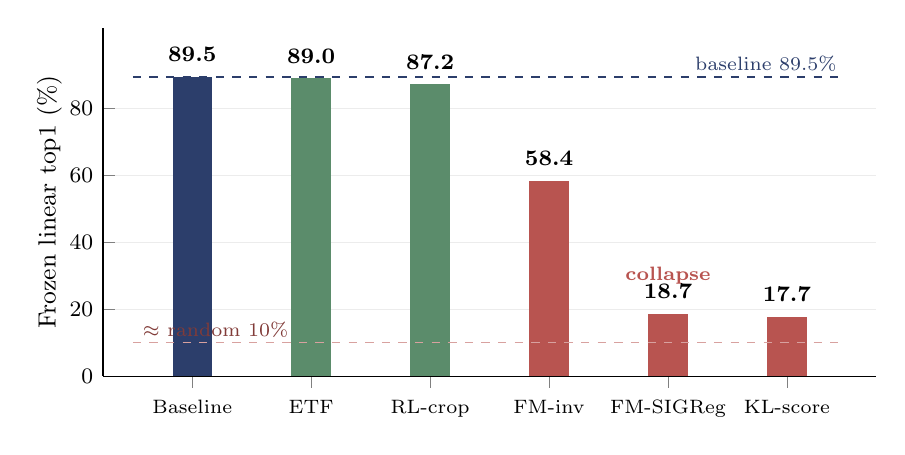
\begin{tikzpicture}
\begin{axis}[
    width=11.4cm, height=6.0cm,
    clip=false,
    ybar, bar width=0.5cm,
    ylabel={Frozen linear top1 (\%)},
    ylabel style={yshift=-4pt},
    ymin=0, ymax=104,
    ytick={0,20,40,60,80},
    ymajorgrids=true,
    grid style={mgray!20},
    axis x line*=bottom,
    axis y line*=left,
    xmin=-0.75, xmax=5.75,
    xtick={0,1,2,3,4,5},
    xticklabels={Baseline,ETF,RL-crop,FM-inv,FM-SIGReg,KL-score},
    xticklabel style={font=\scriptsize, yshift=-1pt},
    tick label style={font=\footnotesize},
    label style={font=\small},
    nodes near coords,
    point meta=explicit symbolic,
    nodes near coords style={font=\footnotesize\bfseries, yshift=2pt},
    bar shift=0pt]
  % control group (objective untouched) -> sage
  \addplot[draw=none, fill=mprimary] coordinates {(0,89.49) [89.5]};
  \addplot[draw=none, fill=mgood]    coordinates {(1,89.02) [89.0]};
  \addplot[draw=none, fill=mgood]    coordinates {(2,87.20) [87.2]};
  % objective-swap group -> terracotta
  \addplot[draw=none, fill=mbad]     coordinates {(3,58.42) [58.4]};
  \addplot[draw=none, fill=mbad]     coordinates {(4,18.68) [18.7]};
  \addplot[draw=none, fill=mbad]     coordinates {(5,17.68) [17.7]};
  % baseline anchor
  \draw[mprimary, thick, dashed] (axis cs:-0.5,89.49) -- (axis cs:5.5,89.49);
  \node[font=\scriptsize, mprimary, anchor=east] at (axis cs:5.5,93.5) {baseline 89.5\%};
  % random floor
  \draw[mbad!55, dashed] (axis cs:-0.5,10) -- (axis cs:5.5,10);
  \node[font=\scriptsize, mbad!70!black, anchor=west] at (axis cs:-0.5,14) {$\approx$ random 10\%};
  % collapse annotation over the swap cluster
  \node[font=\scriptsize\bfseries, mbad, align=center] at (axis cs:4,30) {collapse};
\end{axis}
\end{tikzpicture}
\end{document}
